\section{Laboratory work implementation} 

\subsection{The chosen program}
\begin{lstlisting}
	#include <stdio.h>
	#include <string.h>
	#include <algorithm>
	
	using namespace std;
	
	int main() {
	
		int T;
		scanf("%d",&T);
	
		while (T--) {
			int X, Sol = 0;
			scanf("%d",&X);
			
			while (X--) {
				int Y;
				scanf("%d",&Y);
				Sol ^= Y;
			}
	
			if (Sol)
				printf("DA\n");
			else
				printf("NU\n");
		}
	
		return 0;
	}
\end{lstlisting}

\subsection{Task 1 - Graph of the control flow}

\begin{center}
	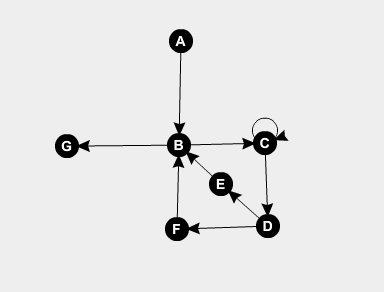
\includegraphics[scale=1]{images/Capture2}
	\captionof{figure}{Graph of the control flow}
	\vspace{1cm}
\end{center}

\begin{itemize}
	\item A - is the initial state, before we enter the \textbf{while (T--)} loop;
	\item B - is the start of the first while loop;
	\item C - comes from B and is the start of the second loop, it has self edge to represent the inner while loop;
	\item D - is the if statement from which we can get to E or F;
	\item E, F - different statements depending on if statement and from them we start a new iteration to B;
	\item G - is the end of the program;
\end{itemize}


\subsection{Task 2 - Test the program according to the coverage criteria}

a) All instruction coverage :

\vspace{0.5cm} 

T = 2; 

X1 = 1; 

Y1[] = {10}; 

X2 = 0; 

Y2[] = {};

\vspace{0.5cm} 

For this test case all the statements are traversed at least once, hence each line is tested, as far as we know!!
\vspace{1cm}


b) All edges coverage :

\vspace{0.5cm}

T = 2; 

X1 = 2; 

Y1[] = {10, 2}; 

X2 = 0; 

Y2[] = {};

\vspace{0.5cm}

To traverse each edge at least once I've added a number for the first array so that the self loop could be traversed, now all edges have been checked;

\vspace{1cm}


c) All simple conditions coverage :

\vspace{0.5cm}

For the conditional part in my program I have only one if statement where I check if \textbf{Sol} variable is 0 or not. In the previous cases I've covered both of them;

\vspace{1cm}


d) All paths coverage : 

\vspace{0.5cm}

T = 2; 

X1 = 2; 

Y1[] = {10, 2}; 

X2 = 2; 

Y2[] = {10, 10};

\vspace{0.5cm}

To cover all the possible paths I've added an array with length longer than 1 to have the first while loop to perform more than 1 iteration and the program works as expected;

\vspace{1cm} 


\subsection{Task 3 - Samples with erroneous results}

I didn't met any samples to produce erroneous results. The only samples that could do so are those in which T or X are negative. 

This way my program falls into infinite loop because I didn't check the values to be positive, but it is contrary to the constraints of the problem solved by the program.

\subsection{Task 4 - Comments}

\begin{itemize}
	\item As I said previously my program falls for negative values, and thats because the iterators are only decremented and tested to be not zero but not positive;
	\item There are not some complex conditional samples because I have only one if statement with one condition which leads to 2 possibilities;
	\item Out of the four coverage methods I consider the third i.e. for the simple conditions one with a good performance and good coverage, yet it has exceptions as proven when we have more conditions;
\end{itemize}


\subsection{Task 5 - McCabe technique}

\begin{itemize}
	\item $Nr_{C} = E - V + 2 = 9 - 7 + 2 = 4;$
	\item The paths : 
		  \begin{itemize}
		      \item A $\rightarrow$ B $\rightarrow$ C $\rightarrow$ D $\rightarrow$ E $\rightarrow$ B $\rightarrow$ G;
		      \item A $\rightarrow$ B $\rightarrow$ C $\rightarrow$ D $\rightarrow$ F $\rightarrow$ B $\rightarrow$ G;
		      \item A $\rightarrow$ B $\rightarrow$ C $\rightarrow$ C $\rightarrow$ D $\rightarrow$ E $\rightarrow$ B $\rightarrow$ G;
		      \item A $\rightarrow$ B $\rightarrow$ G;
		  \end{itemize}
	\item The test cases : 
		  \begin{itemize}
		  	  \item T = 1; 
		  	  
		  	  		X1 = 1; 
		  	  
		  	  		Y1[] = {10}; 
		  	  		
		  	  \item T = 1; 
		  	  
			  	    X1 = 1; 
			  	  
			  	    Y1[] = {0};
			  	    
			  \item T = 1; 
			  
			  		X1 = 2; 
			  
	   			    Y1[] = {0, 0}; 
	   			    
	   		  \item T = 0;
		  	  
		  \end{itemize}
	  
	\item After checking the tests the program worked as expected;	 	
	
\end{itemize}